\section{Der grundlegende Aufbau einer Android App}
Im nun folgenden Kapitel wird der grundlegende Aufbau einer Android App genauer beschrieben, wobei auf wichtige Bestandteile im Projekt eingegangen wird.
Zum einen soll hier der zugrundeliegende Dateiaufbau aber auch die Bestandteile einer App und deren Funktion genauer erl\"autert dargestellt werden.

\subsection{Componenten einer Applikation aus Sicht des Nutzers}
Eine App unter Android bestizt aus der sicht des Nutzers vier Hauptbestandteile:
\begin{itemize}
 \item Activity
 \item BroadcastReceiver
 \item Service
 \item ContentProvider
\end{itemize}

\subsubsection{Die Activity}
Eine Activity, unter Android, ist eine Benutzeroberfl\"ache in der App, wobei ein Projekt beliebig viele Activitys haben kann. Somit sind Activitys im eigentlichen Sinn Fenster, die in der Regel den gesamten Bildschirm f\"ullen und eine gewisse Aufgabe erf\"ullen. \cite{Kuehn12}

Der Aufruf verschiedener Activitys kann entweder vom Programmablauf vorgegeben sein oder durch Nutzeraktionen variieren. So kann zum Beispiel jenachdem welchen Button der Nutzer bet\"atigt eine andere Activity aufgerufen werden. \cite{Android44}

Eine Activity hat einen bestimmten Lebenszyklus den sie im Verlauf der Anwendung durchl\"auft. Beim erstellen einer Activity wird als erstes die Methode \texttt{onCreate} aufgerufen. Jenachdem welche Folgeaktion der Nutzer als n\"achstes ausf\"uhrt wird eine der Anderen Methoden wie im Bild \ref{ActivityLebenszyklus} aufgerufen. Wird die Activity wieder beendet, so wird die Methode \texttt{onDestroy} aufgerufen. 

Inaktiv ist eine Activity zum Beispiel dann, wenn die von einer anderen komplett oder Teilweise \"uberdeckt wird. Sollte eine neue Activity \"uber der alten ge\"offnet werden, wird diese nicht sofort zerst\"ort, sondern auf einer Art Stack gehalten von woaus sie wieder aufgerufen werden kann. Dies w\"are der Fall, wenn der Nutzer die Zur\"ucktaste bet\"atigt.

Activitys die sich im Stack befinden, werden erst gel\"oscht, wenn die zugeh\"orige App geschlossen oder Arbeitsspeicher freigegeben werden muss. 

Alle im Bild \ref{ActivityLebenszyklus} zu sehenden Methoden sind unten in Tabelle \ref{Lebenszyklus-Methode einer Activity} noch einmal genauer beschrieben.

\begin{figure}[!ht]
\centering
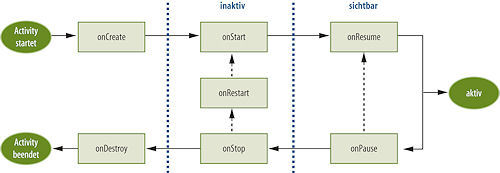
\includegraphics[width=12cm]{Bilder/ActivityLifecycle}
\caption{Der Lebenszyklus einer Activity \cite{ActivityLifecycle}}
\label{ActivityLebenszyklus}
\centering
\end{figure}

In der folgenden Tabelle sind alle m\"oglichen Methoden beschrieben, welche im Lebenszyklus einer Activity vom Betriebssystem aufgerufen werden k\"onnen.

\begin{table}
\begin{tabular}{|p{3cm}|p{12cm}|}
 \hline Methode & Beschreibung \\
 \hline onCreate & Diese Methode wird beim erzeugen der Activity aufgerufen und kann wie ein Konstruktor verwendet werden. Es werden alle Felder, Formulare, Men\"us und Layouts hier initialisiert.\\&\\
 onStart & Wird ausgef\"uhrt, wenn die Activity neu erzeugt wird oder sie aus dem Hintergrund wieder hervortritt, wie es zum Beispiel beim dr\"ucken der Zur\"ucktaste der Fall ist.\\&\\
 onResume & Wenn eine teilweise verdeckte Activity wieder in den Focus r\"uckt wird diese Methode Aufgerufen.\\&\\
 on Pause & Diese Methode wird Ausgef\"uhrt, wenn die Activity teilweise verdeckt wird und somit inaktiv wird.\\&\\
 onStop & Wird ausgef\"uhrt, wenn die Activity in den Hintergrund tritt und auf den Stack abgelegt wird.\\&\\
 onRestart & Die Activity r\"uckt vom Stack wieder in den Vordergrund weil diese wieder ben\"otigt wird\\&\\
 onDestroy & Diese Methode wird ausgef\"uhrt, wenn die Activity beendet wird. In ihr sollten alle belegten Ressourcen wieder freigegeben werden.\\
 \hline
\end{tabular}
\caption{Lebenszyklus-Methode einer Activity \cite{Android44}}
\label{Lebenszyklus-Methode einer Activity}
\end{table}